\section{Diskrete Fouriertransformation (DFT)}

Die \gls{dft} ist die zeit- und wertdiskrete Variante der Fouriertransformation, die statt von $-\infty$ bis $\infty$ über einen Vektor von N Werten, also von 0 bis N-1 läuft. 
Dies hat zur Folge, dass sich ihr Frequenzspektrum periodisch nach N Werten wiederholt.

Da es sich um eine endliche Anzahl diskreter Werte handelt, geht das Integral aus Gleichung (\ref{eq:Fouriertransformation}) in die Summe aus Gleichung (\ref{eq:dft}) über. 


Üblicher Weise wird die (diskrete) Fouriertransformation genutzt, um vom Zeitbereich in den Frequenzbereich zu gelangen. In diesem Fall enthielte der Eingangsvektor 
Werten im Zeitbereich, der Ausgangsvektor Werten im Frequenzbereich.
Um von Daten im Zeitbereich sprechen zu können, müssen diese zeitliche versetzt auf den gleichen Bezugspunkt erfasst worden sein. 
Bezogen auf das Sensorarray würde eine bestimmte Anzahl an zeitlich versetzten zeit- und wertdiskretisierten Daten eines einzelnen Sensors in einem Vektor zusammengefasst 
und darauf die \gls{dft} angewandt werden, um beim Ausgangsvektor von Daten im Frequenzbereich sprechen zu können.

Statt zeitlich versetzter Daten werden beim Sensorarray die Daten von mehreren Sensoren gleichzeitig erfasst. Da das Sensorarray zweidimensional ist, ergibt
sich an Stelle eines Vektors so eine Matrix. Weil die Werte gleichzeitig erfasst werden und diese verschiedene Koordinaten repräsentieren, muss hier von Orts- anstatt von
Zeitwerten gesprochen werden. Von der Transformation ins Frequenzspektrum spricht man wiederum bei Zeitwerten, da das Spektrum die Frequenzen darstellt, aus denen das Zeitsignal 
zusammengesetzt ist. Da bei der eben beschriebenen Datenerfassung Ortsdaten transformiert werden, spricht man hier allgemeiner von einer Transformation in den Bilbereich. 

In dieser Arbeit werden statt Zeit- bzw. Ortsbereich respektive Frequenzbereich und Bildverarbeitung häufig auch die Begriffe Ein- und Ausgangsvektor bzw. -matrix verwendet.

Mit der \gls{1d-dftn} wird die spaltenweise DFT einer Matrix bezeichnet, in der Regel ist sie der erste Schritt der Berechnung der \gls{2d-dft}. 
Die Größe der Eingangsmatrix gibt die Größe der Twiddlefaktormatrix vor, beide müssen identisch und
quadratisch sein. In dieser Arbeit wird die \gls{dft} einer Matrix der Größe $N$x$N$ auch $N$x$N$-\gls{dft} genannt.


\subsection{Summen- und Matrizenschreibweise der DFT}
\subsubsection{1D-DFT}
Die \gls{dft} findet wie bereits erwähnt üblicherweise Anwendung, um vom Zeit- in den Frequenzbereich zu gelangen.
\begin{equation}\label{eq:dft}
 X^* \left[ m \right] = \frac{1}{N} \cdot \sum^{N-1}_{n=0} x[n] \cdot e^{-\frac{j 2 \pi m n}{N}}
\end{equation}


In Gleichung (\ref{eq:dft}) ist die übliche Verwendung von Eingangsvektor $x[n]$ und Ausgangsvektor $X[n]$ zu sehen. Eine spaltenweise Multiplikationen einer Matrix
ist auch denkbar und ist darüber hinaus Grundlage für die \gls{2d-dft}.
Gleichung (\ref{eq:1D-DFT_MatrixMult}) zeigt die Summenformel aus (\ref{eq:dft}) umgeschrieben zu einer Matrixmultiplikation.

Mit Gleichung (\ref{eq:Twiddlefaktorenberechnung}) werden zunächst alle Twiddlefaktoren in Matrixform berechnet, wobei $n$ der Index des zu Berechnenden Elements des 
Vektors im Zeitbereich und $m$ das Äquivalent im Frequenzbereich ist.

\begin{equation}\label{eq:Twiddlefaktorenberechnung}
\sum^{N-1 }_{m=0} \sum^{N-1 }_{n=0} e^{-\frac{j 2 \pi m n}{N}} = W
\end{equation}


Somit gilt:

\begin{equation}\label{eq:1D-DFT_MatrixMult}
X^* = W \cdot x
\end{equation}

In Matlab kann die Twiddlefaktormatrix mit
\begin{equation}\label{eq:matlab_dft_faktoren}
 W = e^{-\frac{i 2 \pi}{N}\cdot[0:N-1]'\cdot[0:N-1]}
\end{equation}
berechnet werden, wobei N die Anzahl der Elemente je Zeile bzw. Spalte ist.


\subsubsection{2D-DFT}
Die \gls{2d-dft} wird hingegen häufig in der Bildverarbeitung verwendet, um vom Orts- in den Fourierraum zu gelagen. Da es sich somit nicht mehr um eine Abhänigkeit 
der Zeit handelt, werden andere Indizes verwendet.
\begin{align}
\begin{split}
X[u,v] 	&= \frac{1}{N} \sum^{N-1}_{n=0} X^* \left[ m \right] \cdot e^{-\frac{j 2 \pi m n}{N}}\\
	&= \frac{1}{MN} \sum^{M-1}_{m=0} \left( \sum^{N-1}_{n=0} f(m,n) \cdot e^{-\frac{j 2 \pi m n}{N}} \right) \cdot e^{-\frac{j 2 \pi m n}{M}}
\end{split}
\end{align}

Auch hier lässt sich die Berechnung in Matrizenschreibweise darstellen:

\begin{align}
\begin{split}\label{eq:2D-DFT_MatrixMult}
 X &= W \cdot x \cdot W \\
                    &= X^* \cdot W
\end{split}
\end{align}

Die Gleichungen (\ref{eq:1D-DFT_MatrixMult}) und (\ref{eq:2D-DFT_MatrixMult}) werden wesentlicher Bestandteil der Umsetzung der 2D-DFT sein.
% Die Matrizenmultiplikation aus den genannten Gleichung werden nachfolgend zur Veranschaulichung  grafisch dargestellt, wobei im einen Fall $x$ und im anderen 
% $X^*$ die Eingangsmatrix ist. Bei $W$ handelt es sich um die Twiddlefaktormatrix.
% 
%   
%  \[
%   \stackrel{\mbox{$X^* \quad (X)$}}{
%    \begin{bmatrix}
%     \myBlackBox 	& \myBlackBox 		& \myBlackBox 		& \myBlackBox \\
%     \myDarkgrayBox 	& \myDarkgrayBox 	& \myDarkgrayBox 	& \myDarkgrayBox \\
%     \myGrayBox 		& \myGrayBox 		& \myGrayBox 		& \myGrayBox \\
%     \myLightgrayBox 	& \myLightgrayBox 	& \myLightgrayBox 	& \myLightgrayBox 
%    \end{bmatrix}
%   }
%   =
%   \stackrel{\mbox{$W \quad (X^*)$}}{
%    \begin{bmatrix}
%     \myBlackBox 	& \myBlackBox 		& \myBlackBox 		& \myBlackBox \\
%     \myDarkgrayBox 	& \myDarkgrayBox 	& \myDarkgrayBox 	& \myDarkgrayBox \\
%     \myGrayBox 		& \myGrayBox 		& \myGrayBox 		& \myGrayBox \\
%     \myLightgrayBox 	& \myLightgrayBox 	& \myLightgrayBox 	& \myLightgrayBox 
%    \end{bmatrix}
%   }
%   \cdot
%   \stackrel{\mbox{$x \quad (W)$}}{
%    \begin{bmatrix}
%     \myBlackBox & \myBlackBox & \myBlackBox & \myBlackBox \\
%     \myBlackBox & \myBlackBox & \myBlackBox & \myBlackBox \\
%     \myBlackBox & \myBlackBox & \myBlackBox & \myBlackBox \\
%     \myBlackBox & \myBlackBox & \myBlackBox & \myBlackBox 
%    \end{bmatrix}
%   }
%  \]

 
%  \[
%   \stackrel{\mbox{$X$}}{
%    \begin{bmatrix}
%     \myBlackBox 	& \myBlackBox 		& \myBlackBox 		& \myBlackBox \\
%     \myDarkgrayBox 	& \myDarkgrayBox 	& \myDarkgrayBox 	& \myDarkgrayBox \\
%     \myGrayBox 		& \myGrayBox 		& \myGrayBox 		& \myGrayBox \\
%     \myLightgrayBox 	& \myLightgrayBox 	& \myLightgrayBox 	& \myLightgrayBox 
%    \end{bmatrix}
%   }
%   =
%   \stackrel{\mbox{$X^*$}}{
%    \begin{bmatrix}
%     \myBlackBox 	& \myBlackBox 		& \myBlackBox 		& \myBlackBox \\
%     \myDarkgrayBox 	& \myDarkgrayBox 	& \myDarkgrayBox 	& \myDarkgrayBox \\
%     \myGrayBox 		& \myGrayBox 		& \myGrayBox 		& \myGrayBox \\
%     \myLightgrayBox 	& \myLightgrayBox 	& \myLightgrayBox 	& \myLightgrayBox 
%    \end{bmatrix}
%   }
%   \cdot
%   \stackrel{\mbox{$W$}}{
%    \begin{bmatrix}
%     \myBlackBox & \myBlackBox & \myBlackBox & \myBlackBox \\
%     \myBlackBox & \myBlackBox & \myBlackBox & \myBlackBox \\
%     \myBlackBox & \myBlackBox & \myBlackBox & \myBlackBox \\
%     \myBlackBox & \myBlackBox & \myBlackBox & \myBlackBox 
%    \end{bmatrix}
%   }
%  \]



Wie in Gleichung (\ref{eq:2D-DFT_MatrixMult}) beschrieben, kann die 2D-DFT als ``doppelte'' Matrizenmultiplikation geschrieben werden.
Es wird also erst die 1D-DFT berechnet und die sich daraus ergebende Matrix $X^*$ (Abb. \ref{eq:matrix_F1}) wird anschließend mit der Twiddlefaktor-Matrix $W$ 
multipliziert. Man könnte es auch als zweite 1D-DFT betrachten, bei der Twiddlefaktor-Matrix und Eingangsmatrix vertauscht sind.

Veranschaulicht wird dies in den Abbildungen \ref{eq:matrix_F1} und \ref{eq:matrix_F2}.


\begin{center}
 
\begin{minipage}{0.2\textwidth}
 \begingroup
 \renewcommand*{\arraystretch}{1.1} % Zeilenabstand
 \renewcommand*{\arraycolsep}{0.0pt} % Spaltenabstand

 \[
  \stackrel{\mbox{$W$}}{
   \begin{bmatrix}
    \myBlackBox 	& \myBlackBox 		& \myBlackBox 		& \myBlackBox \\
    \myLightgrayBox 	& \myLightgrayBox 	& \myLightgrayBox 	& \myLightgrayBox \\
    \myLightgrayBox 	& \myLightgrayBox	& \myLightgrayBox	& \myLightgrayBox \\
    \myLightgrayBox 	& \myLightgrayBox 	& \myLightgrayBox 	& \myLightgrayBox 
   \end{bmatrix}
  }
 \]
 \endgroup
\end{minipage}
\begin{minipage}{0.05\textwidth}
 \[
  \cdot
 \]
\end{minipage}
\begin{minipage}{0.2\textwidth}
 \begingroup
 \renewcommand*{\arraystretch}{0.0} % Zeilenabstand
 \renewcommand*{\arraycolsep}{0.8pt} % Spaltenabstand

 \[
  \stackrel{\mbox{$x$}}{
   \begin{bmatrix}
    \myBlackBoxHigh 	& \myBlackBoxHigh 	& \myBlackBoxHigh 	& \myBlackBoxHigh \\
    \myBlackBoxHigh 	& \myBlackBoxHigh 	& \myBlackBoxHigh 	& \myBlackBoxHigh \\
    \myBlackBoxHigh 	& \myBlackBoxHigh 	& \myBlackBoxHigh 	& \myBlackBoxHigh \\
    \myBlackBoxHigh 	& \myBlackBoxHigh 	& \myBlackBoxHigh 	& \myBlackBoxHigh 
   \end{bmatrix}
  }
 \]
 \endgroup
\end{minipage}
\begin{minipage}{0.05\textwidth}
 \[
  =
 \]
\end{minipage}
\begin{minipage}{0.3\textwidth}
\begingroup
\renewcommand*{\arraystretch}{1.1} % Zeilenabstand
\renewcommand*{\arraycolsep}{0.8pt} % Spaltenabstand
\begin{align}\label{eq:matrix_F1}
  \stackrel{\mbox{$X^*$}}{
   \begin{bmatrix}
    \myBlackBox 	& \myBlackBox 		& \myBlackBox 		& \myBlackBox \\
    \myLightgrayBox 	& \myLightgrayBox 	& \myLightgrayBox 	& \myLightgrayBox \\
    \myLightgrayBox 	& \myLightgrayBox 	& \myLightgrayBox 	& \myLightgrayBox \\
    \myLightgrayBox 	& \myLightgrayBox 	& \myLightgrayBox 	& \myLightgrayBox 
   \end{bmatrix}
  }
\end{align}

 
 \endgroup
\end{minipage}
\end{center}


\begin{center}
 
\begin{minipage}{0.2\textwidth}
 \begingroup
 \renewcommand*{\arraystretch}{1.1} % Zeilenabstand
 \renewcommand*{\arraycolsep}{0.0pt} % Spaltenabstand

 \[
  \stackrel{\mbox{$X^*$}}{
   \begin{bmatrix}
    \myBlackBox 	& \myBlackBox 		& \myBlackBox 		& \myBlackBox \\
    \myLightgrayBox 	& \myLightgrayBox 	& \myLightgrayBox 	& \myLightgrayBox \\
    \myLightgrayBox 	& \myLightgrayBox	& \myLightgrayBox	& \myLightgrayBox \\
    \myLightgrayBox 	& \myLightgrayBox 	& \myLightgrayBox 	& \myLightgrayBox 
   \end{bmatrix}
  }
 \]
 \endgroup
\end{minipage}
\begin{minipage}{0.05\textwidth}
 \[
  \cdot
 \]
\end{minipage}
\begin{minipage}{0.2\textwidth}
 \begingroup
 \renewcommand*{\arraystretch}{0.0} % Zeilenabstand
 \renewcommand*{\arraycolsep}{0.8pt} % Spaltenabstand

 \[
  \stackrel{\mbox{$W$}}{
   \begin{bmatrix}
    \myBlackBoxHigh 	& \myBlackBoxHigh 	& \myBlackBoxHigh 	& \myBlackBoxHigh \\
    \myBlackBoxHigh 	& \myBlackBoxHigh 	& \myBlackBoxHigh 	& \myBlackBoxHigh \\
    \myBlackBoxHigh 	& \myBlackBoxHigh 	& \myBlackBoxHigh 	& \myBlackBoxHigh \\
    \myBlackBoxHigh 	& \myBlackBoxHigh 	& \myBlackBoxHigh 	& \myBlackBoxHigh 
   \end{bmatrix}
  }
 \]
 \endgroup
\end{minipage}
\begin{minipage}{0.05\textwidth}
 \[
  =
 \]
\end{minipage}
\begin{minipage}{0.3\textwidth}
\begingroup
\renewcommand*{\arraystretch}{1.1} % Zeilenabstand
\renewcommand*{\arraycolsep}{0.8pt} % Spaltenabstand
\begin{align}\label{eq:matrix_F2}
  \stackrel{\mbox{$X$}}{
   \begin{bmatrix}
    \myBlackBox 	& \myBlackBox 		& \myBlackBox 		& \myBlackBox \\
    \myLightgrayBox 	& \myLightgrayBox 	& \myLightgrayBox 	& \myLightgrayBox \\
    \myLightgrayBox 	& \myLightgrayBox 	& \myLightgrayBox 	& \myLightgrayBox \\
    \myLightgrayBox 	& \myLightgrayBox 	& \myLightgrayBox 	& \myLightgrayBox 
   \end{bmatrix}
  }
 \end{align}
 \endgroup
\end{minipage}
\end{center}






\subsection{2D-DFT mit rellen Eingangswerten}\label{sec:rein_reelle_dft}
Bei der oben beschriebenen Berechnung können die Eingangssignale auch komplex sein. Da das Ausgangssignal der \gls{1d-dft} unabhängig von den Eingangssignalen in jedem Fall 
komplex ist, kann es dort direkt als Eingangssignal für die komplexe \gls{2d-dft} genutzt werden. 

Es wäre jedoch auch möglich, das komplexe Ausgangssignal der \gls{1d-dft} als zwei von einander unabhängige rein relle Eingangssignale der 2D-DFTs zu betrachten und später 
wieder zusammen zu setzen. Gleiches gilt dann natürlich auch für ein komplexes Eingangssignal, welches ebenfalls in zwei von einander unabhängigen DFTs transformiert werden.
Da bei dieser Umsetzung kein Imaginärteil in die Berechnung der Ergebnisse einfließt, hat sie den Vorteil, dass aus Symmetriegründen die Hälfte der Multiplikationen 
eingespart werden können. Hierbei ist es erforderlich, dass der Imaginärteil der gespiegelten Ergebnisse negiert wird. Abbildung \ref{pic:reelleMatMultRedundanz} zeigt die 
redundanten Werte der DFT. Die grau hinterlegten Felder sind die Multiplikationen der Twiddlefaktormatrix. Es müssen bei der 8x8-DFT also statt 16 nur 8 Multiplikationen
mit rellem Multiplikand und komplexen Multiplkator erfolgen.

Wie bereits beschrieben lässt sich dieses Verfahren auch für komplexe Eingangssignale, deren Real- und Imaginärteil separat von einander mit der DFT transformiert werden, anwenden.
Anschließend müssen die Ergebnisse zusammen gesetzt werden. Wie dies geschieht ist der Abbildung \ref{pic:reelleDFT} zu entnehmen.



In Abbildung \ref{pic:reelleDFT} ist die schematische Berechnung der \gls{2d-dft} eines reellen Eingangssignals zu sehen. 
Um die \gls{2d-dft} eines komplexen Eingangssignals zu berechnen, muss entweder eine identische Einheit für den Imaginärteil vorhanden sein oder noch mehr zeitlich versetzt 
berechnet werden. Die Ergebnisse beider 2D-DFTs müssen identisch zusammengefasst werden, wie es zum Abschluss der einzelnen 2D-DFTs geschehen muss.

\begin{figure}[htbp]
 \centering
   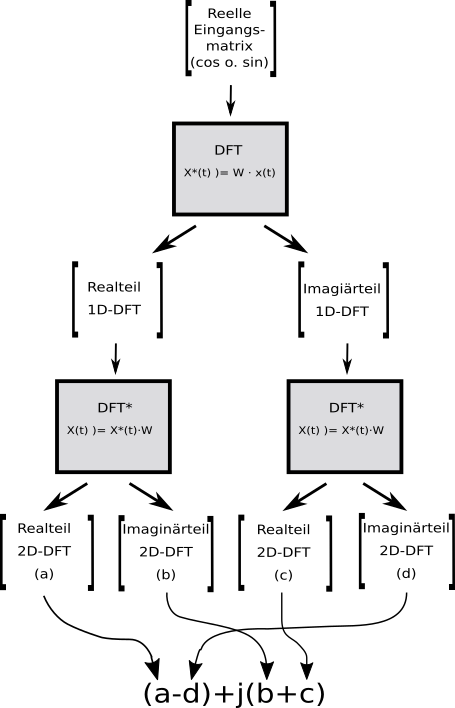
\includegraphics[width=0.6\textwidth]{img/reelleMatMult.png}
 \caption{Veranschaulichung der Berechnung der DFT mit reellen Eingangswerten}
 \label{pic:reelleDFT}
\end{figure}


\begin{figure}[htbp]
 \centering
  \begin{subfigure}{.5\textwidth}
  \centering
   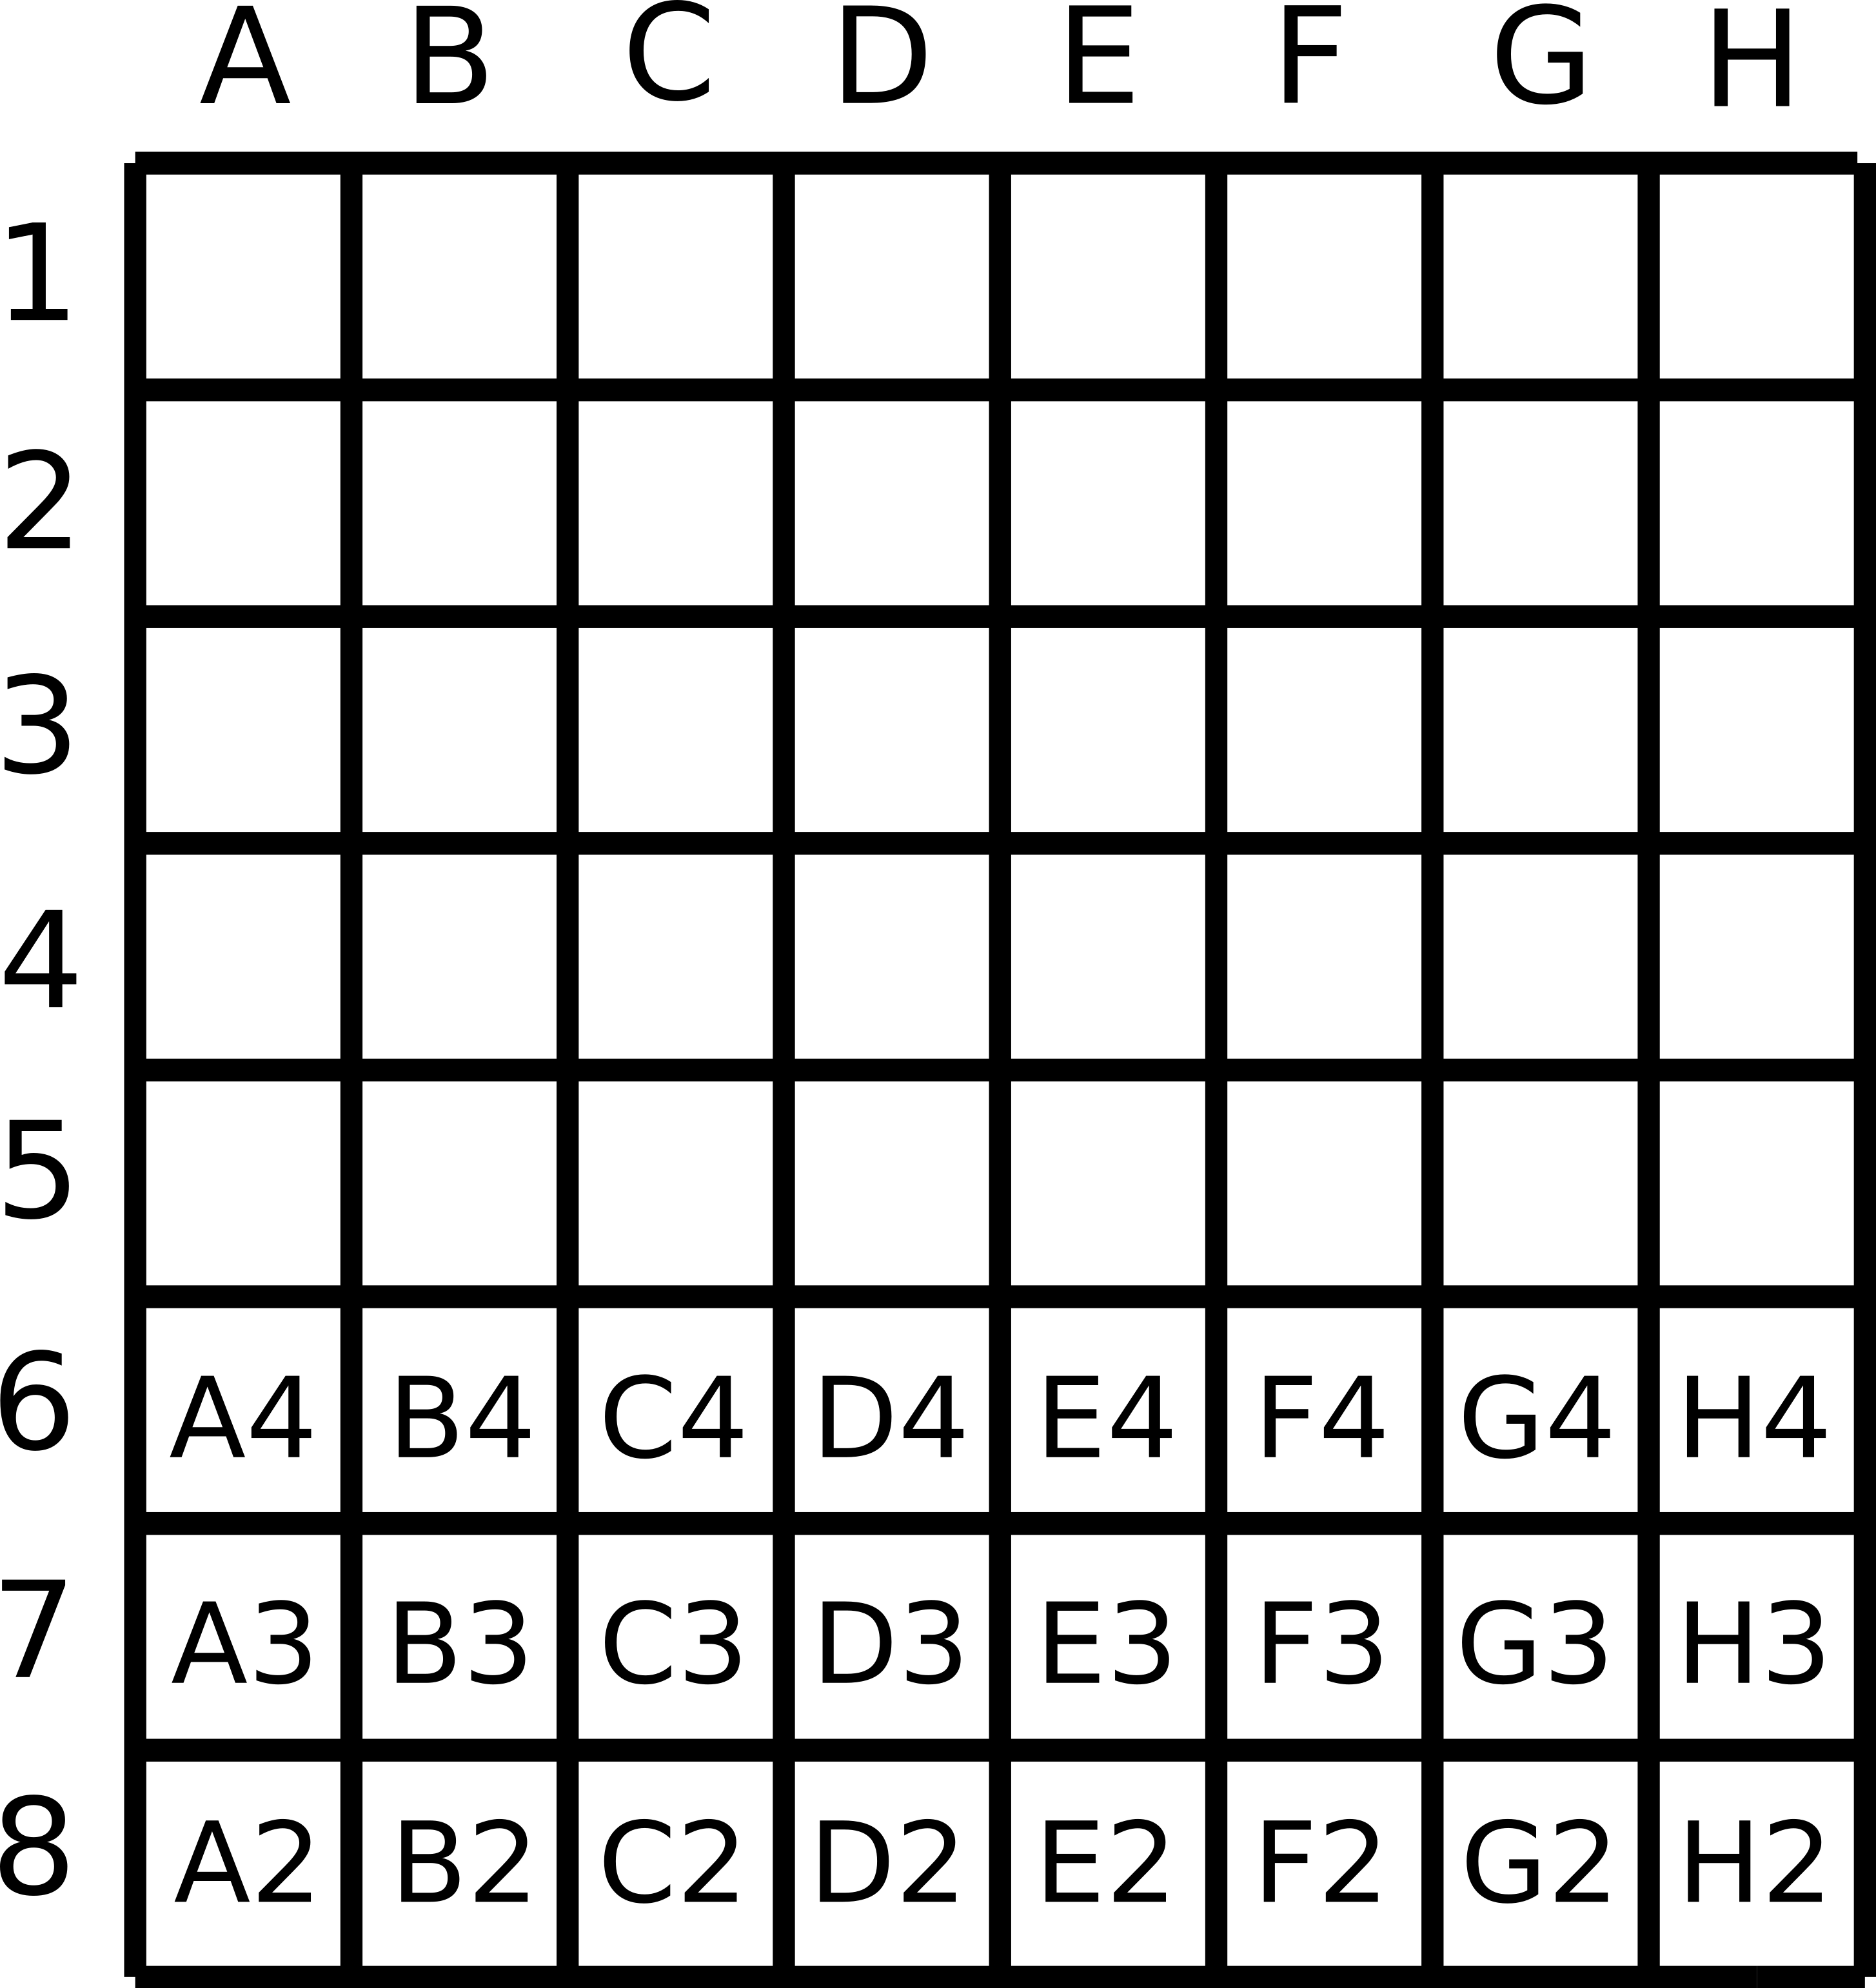
\includegraphics[width=0.8\textwidth]{img/reelleMatMultRedundanzRealteil.png}
   \caption{Realteil}
  \end{subfigure}%
  \begin{subfigure}{.5\textwidth} 
   \centering
   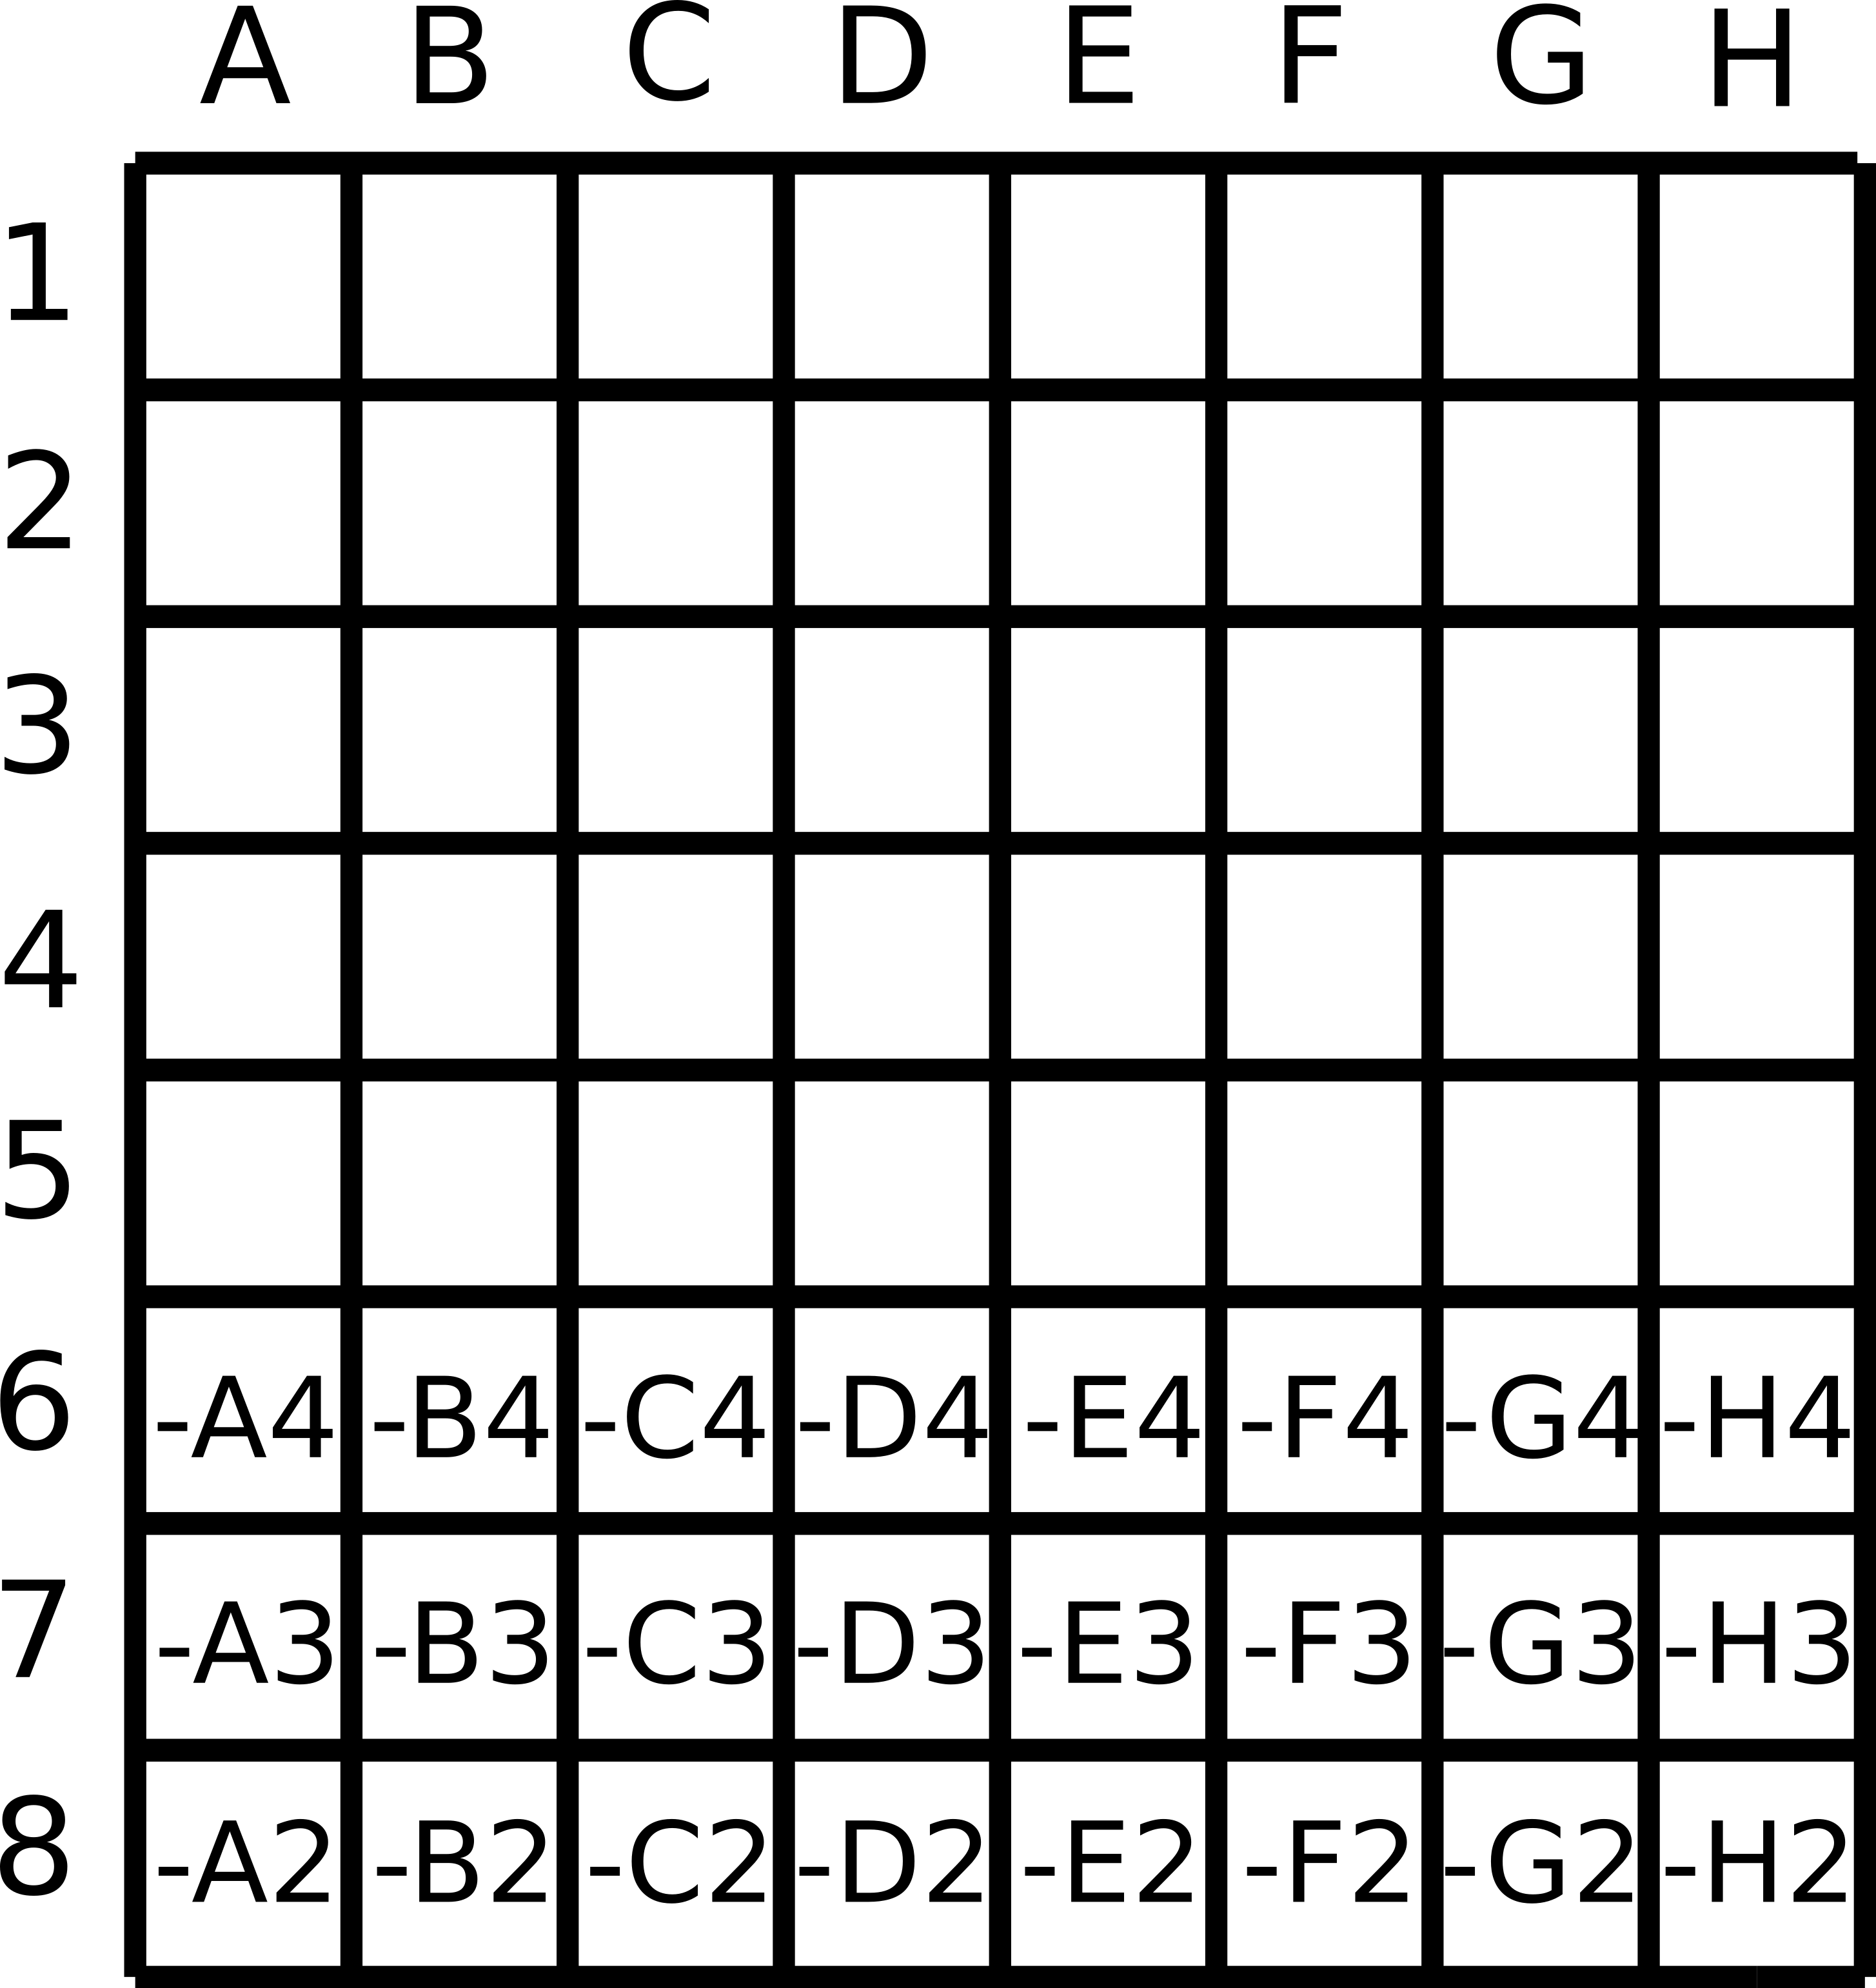
\includegraphics[width=0.8\textwidth]{img/reelleMatMultRedundanzImagteil.png}
   \caption{negierter Imaginärteil}
  \end{subfigure}
  \caption{Redundante Werte der spaltenweisen DFT einer 8x8-Matrix. Der Imaginärteil der redundanten Werte hat den selben Betrag mit negiertem Vorzeichen.}
 \label{pic:reelleMatMultRedundanz}
\end{figure}




Da die gegebenen Eingangssignale aus einer Sinus- und einer Kosinuskomponente bestehen und es sich auf diese Weise als ein komplexes Signal auffassen lässt, kann die 
komplexe Berechnung sowohl bei der 1D-DFT als auch bei der 2D-DFT genutzt werden. 
Da hierdurch in beiden Fällen eine vollständige Auslastung einer komplexen Berechnung gegeben ist und wie bereits erwähnt bei der reellen Berechnung zusätzlicher Speicher 
erforderlich wäre, wird dieses Verfahren angewandt.



